\newgeometry{left=1cm,top=1cm,right=1cm,bottom=1cm} 
\begin{landscape} 
\pagestyle{empty}
\thispagestyle{empty}

% Верхняя "пружина", которая толкает содержимое вниз к центру
\vspace*{\fill}

\begin{center}
    % Вставляем первую страницу
    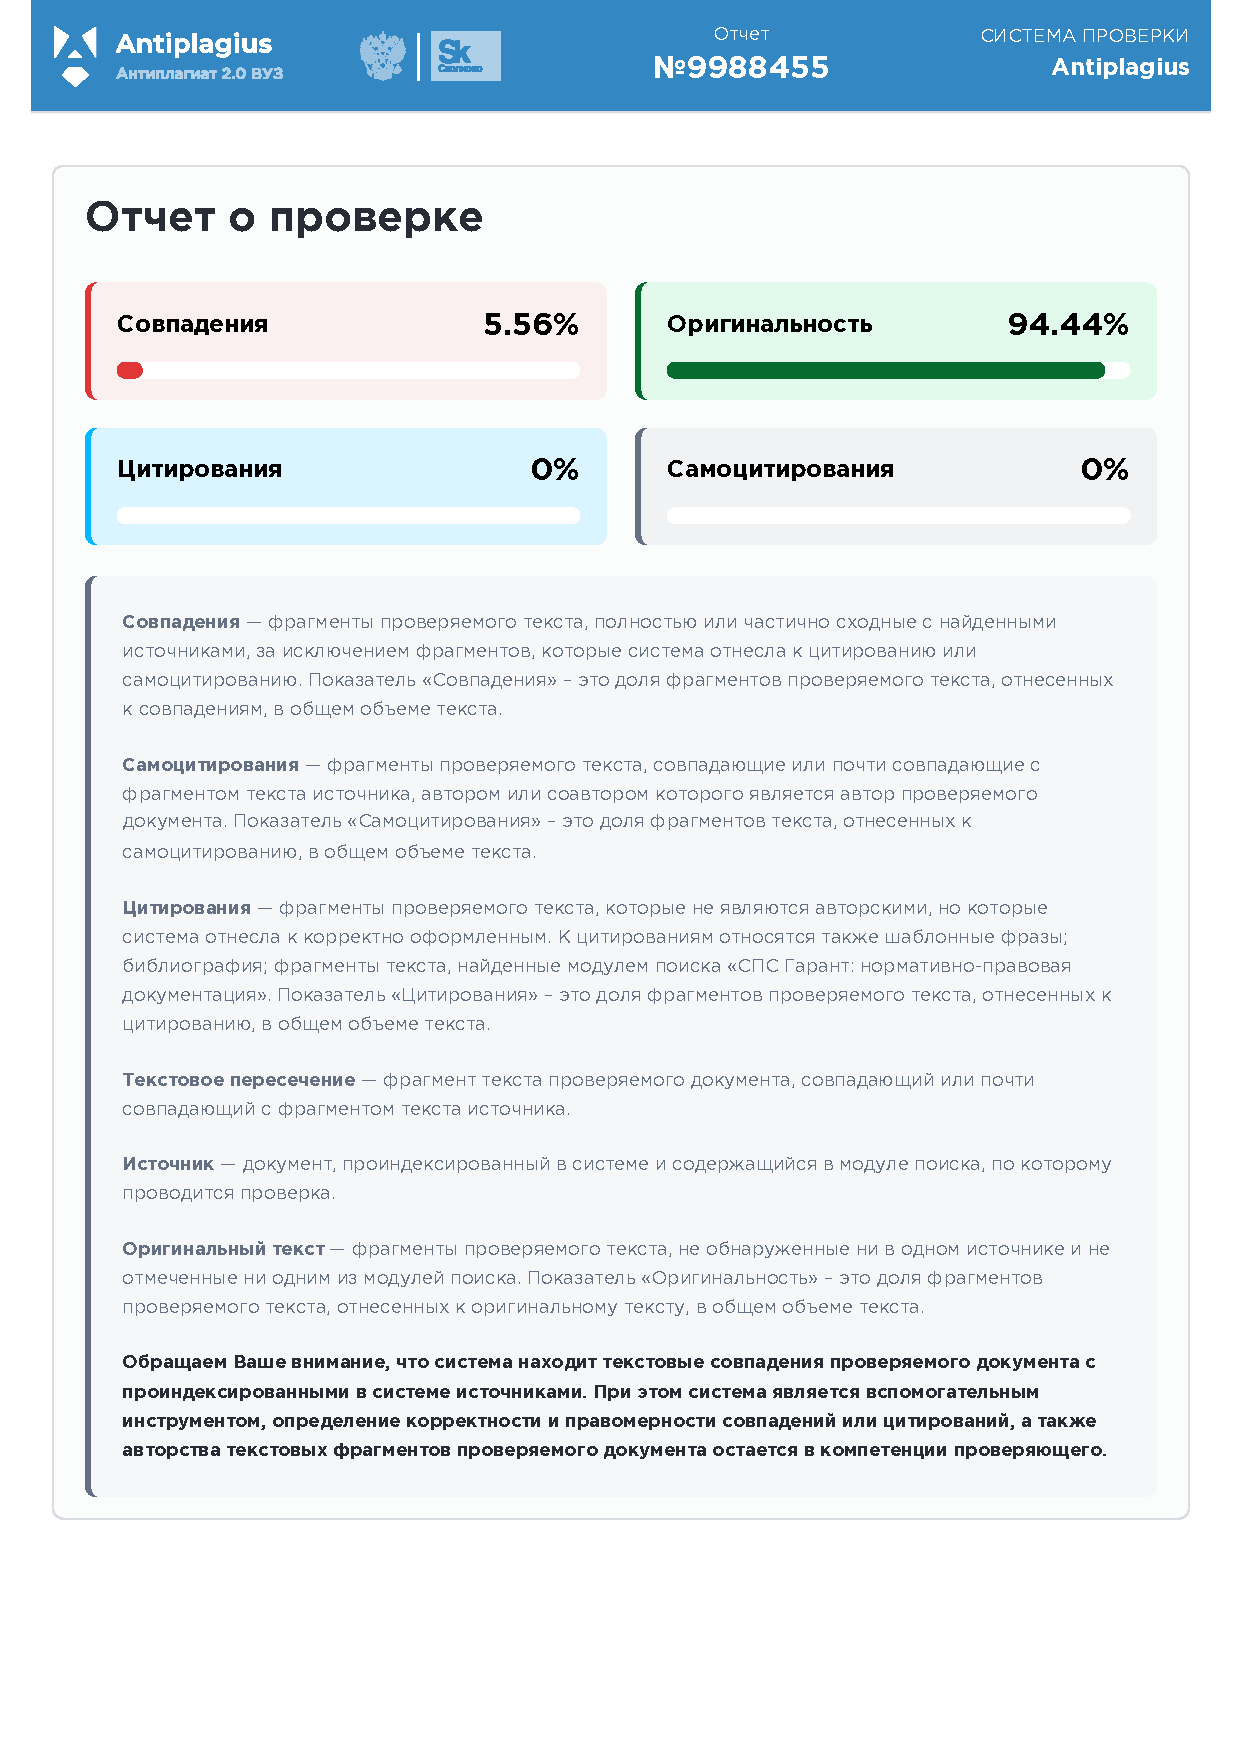
\includegraphics[page=1, width=0.45\linewidth, keepaspectratio]{picture/antiplagius.pdf}%
    % ГОРИЗОНТАЛЬНЫЙ отступ (в твоем коде был \vspace, что ломало высоту)
    \hspace{1cm}%
    % Вставляем вторую страницу
    \includegraphics[page=2, width=0.45\linewidth, keepaspectratio]{picture/antiplagius.pdf}
\end{center}

% Нижняя "пружина", которая толкает содержимое вверх к центру
\vspace*{\fill}

\end{landscape}
\restoregeometry